\documentclass[12pt,a4paper]{article}

\usepackage[utf8]{inputenc}
\usepackage[T1]{fontenc}
\usepackage[english]{babel}
\usepackage{amsmath}
\usepackage{amsfonts}
\usepackage{ae}
\usepackage{units}
\usepackage{icomma}
\usepackage{color}
\usepackage{graphicx}
\usepackage{bbm}
\usepackage{upgreek}
\usepackage{amsthm}
\usepackage{fullpage}
\usepackage{mathtools}
\usepackage{psfrag}
\usepackage{caption}
\usepackage{fancyhdr}
\usepackage[table]{xcolor}
\usepackage{longtable}
\usepackage{hyperref}
\usepackage{tocloft}
\usepackage{epstopdf}
\renewcommand{\cftdotsep}{\cftnodots}
\setlength\parindent{0pt}

\title{IM2601 Solid State Physics \\ Lab exercise 3: Photovoltaic effect: Diode IV-characteristic}

\author{Karl Amundsson karlam@kth.se\\
Alexander Bielik abielik@kth.se\\
Hannes Lindström halinds@kth.se}

\date{\today}

\begin{document}
\maketitle
\thispagestyle{empty}

\newpage

\tableofcontents
\thispagestyle{empty}

\newpage
\setcounter{page}{1}


\section{Introduction}

A solar cell is an electrical device that generates electricity by the photovoltaic effect. Upon exposure to illumination, the device creates voltage, which in turn gives rise to an electric current. Solar cells are becoming increasingly common as an alternative source of electricity. \\

A solar cell can be described as a $p-n$ junction, which is an interface between $p$-type material (acceptors) and $n$-type material (donors) inside a semiconductor. Electrons will diffuse from the $n$-side to the $p$-side, while holes will diffuse from the $p$-side to the $n$-side. At the same time, an electric field comes into existence between the diffused electrons at the $p$-side and the diffused holes at the $n$-side. Whereas the diffusion force pulls electrons to the $n$-side and holes to the $p$-side, the force from the built-in electric field will pull both electrons and holes in the opposite direction, counteracting the diffusion. Sooner or later the forces will be equal, and an equilibrium is established. \\

%\begin{figure}[h]
%\centering
%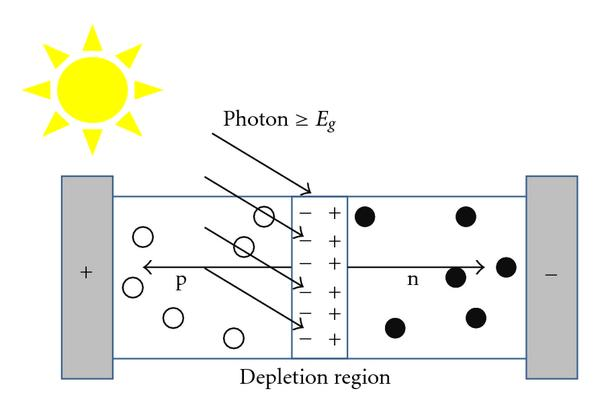
\includegraphics[width=\textwidth]{solarcell.jpg}
%\caption{Basic p-n junction solar cell and charge transport phenomena. (Change description.)}
%\label{fig:solarcell}
%\end{figure}

Free electron-hole pairs can be generated in a semiconductor when it is exposed to light with sufficient energy to excite electrons to the conduction band. If this happens close enough to the interface between the two sides, the electron and hole will feel the built-in electric field, and will consequently be swept in different directions. When the sides are short-circuited, electrons will flow from the $n$-side to the $p$-side to recombine with the holes. This is how solar cells generate an electric current. Note that the direction is the opposite of a diode, because we have minority carriers instead of majority carriers.

\section{Experimental procedure}

We used a thin-film polycrystalline silicon solar cell in this laboratory. By \cite{kittel}, the band gap of silicon is $E_g = 1.11$ eV at $T = 300$ K. It follows that the minimum frequency needed for a monochromatic light source is

$$\nu_g = \frac{E_g}{h} = 2.68 \cdot 10^{14}\text{ Hz,}$$

which corresponds to the wavelength $1100$ nm, which lies in the infrared spectrum. Thus, visible light will be able to drive the solar cell. \\

A Power Cassy was used to apply a selected voltage over the solar cell and measure the current output. The Power Cassy acted as an ideal voltage source. The area of the solar cell was $2.3$ cm $\times$ $6.0$ cm. The solar cell was placed under the light source, a $60$ W desk lamp, at distances varying between $12.5$ cm and $62.5$ cm. \\

We first made a measurement with the lamp turned off and observed that the current was next to zero, as expected; see figure \ref{ivsun} for reference. We next performed a measurement with the lamp turned on and observed a sine curve. This was also expected, since a standard wall outlet outputs an alternating current. \\

We now set the Power Cassy to produce triangular waves with amplitude $57$ V and frequency $0.2$ Hz. Once again, we made measurements with the lamp turned off and then with the lamp turned on. We averaged the current $I_{av}$ over $10$ ms to eliminate the sine like curve due to the wall outlet. \\

We finally measured the power delivered from the solar cell for each of the eleven distances using the relation $P = I_{av} \cdot U$. The power delivered to the surface of the solar cell should theoretically depend on the table-to-lamp distance $d$ by means of the formula $P(d) = \frac{P_0}{(d/d_0)^2}$, where $P_0$ is a reference value at distance $d_0$. We later contemplated the maximal power, which depends on the total radiative power received.

\begin{table}
  \centering
  \begin{tabular}{|c|c|}
    \hline
    Distance [cm] & $P_{max}$ [W] \\
    \hline
    12.5 & 0.07983 \\
    17.5 & 0.05617 \\
    22.5 & 0.04975 \\
    27.5 & 0.04169 \\
    32.5 & 0.03914 \\
    37.5 & 0.03278 \\
    42.5 & 0.02902 \\
    47.5 & 0.02727 \\
    52.5 & 0.02393 \\
    57.5 & 0.02159 \\
    62.5 & 0.02100 \\
    \hline
  \end{tabular}
  \caption{Maximum power for different distances}
  \label{tab}
\end{table}

\newpage
\section{Measurement results}zo
\vfill
\begin{figure}[h!]
  \begin{center}
    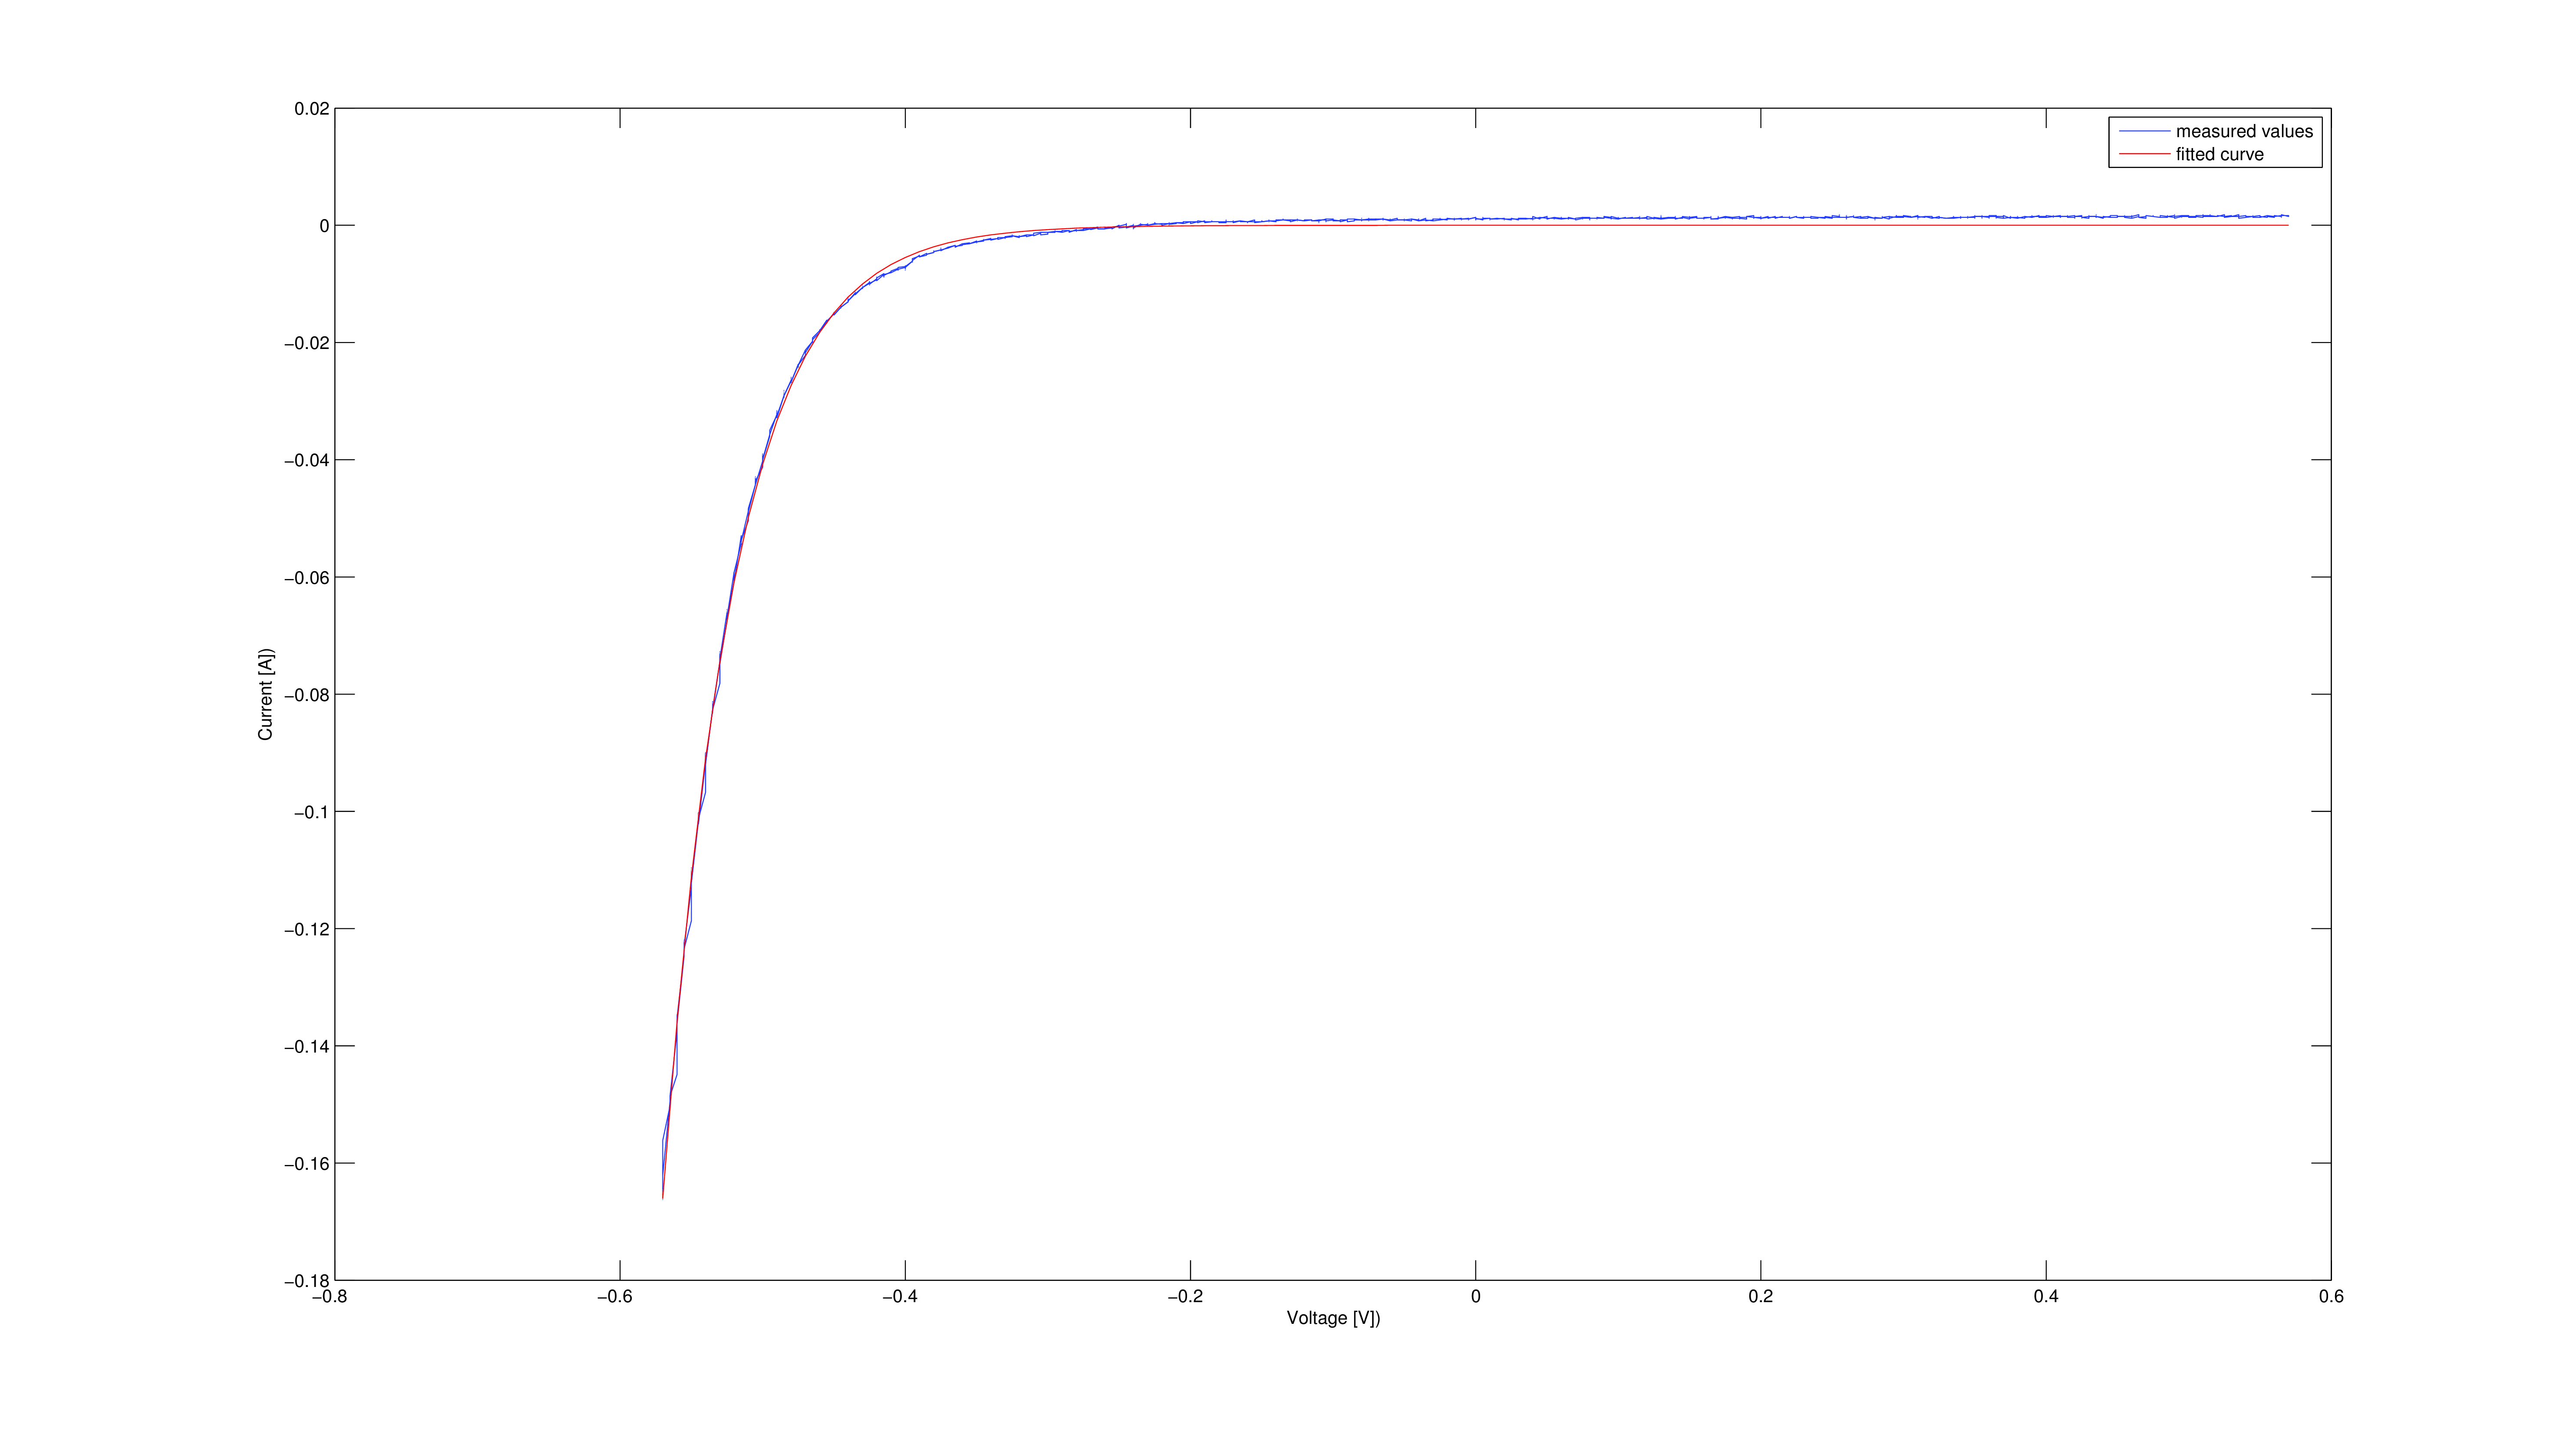
\includegraphics[scale=0.07]{IvsUnoIlumination.png}
  \end{center}
  \caption{Current as function of voltage. Fitted according to the diode equation.}
  \label{ivsun}
\end{figure}

\begin{figure}[h!]
  \begin{center}
    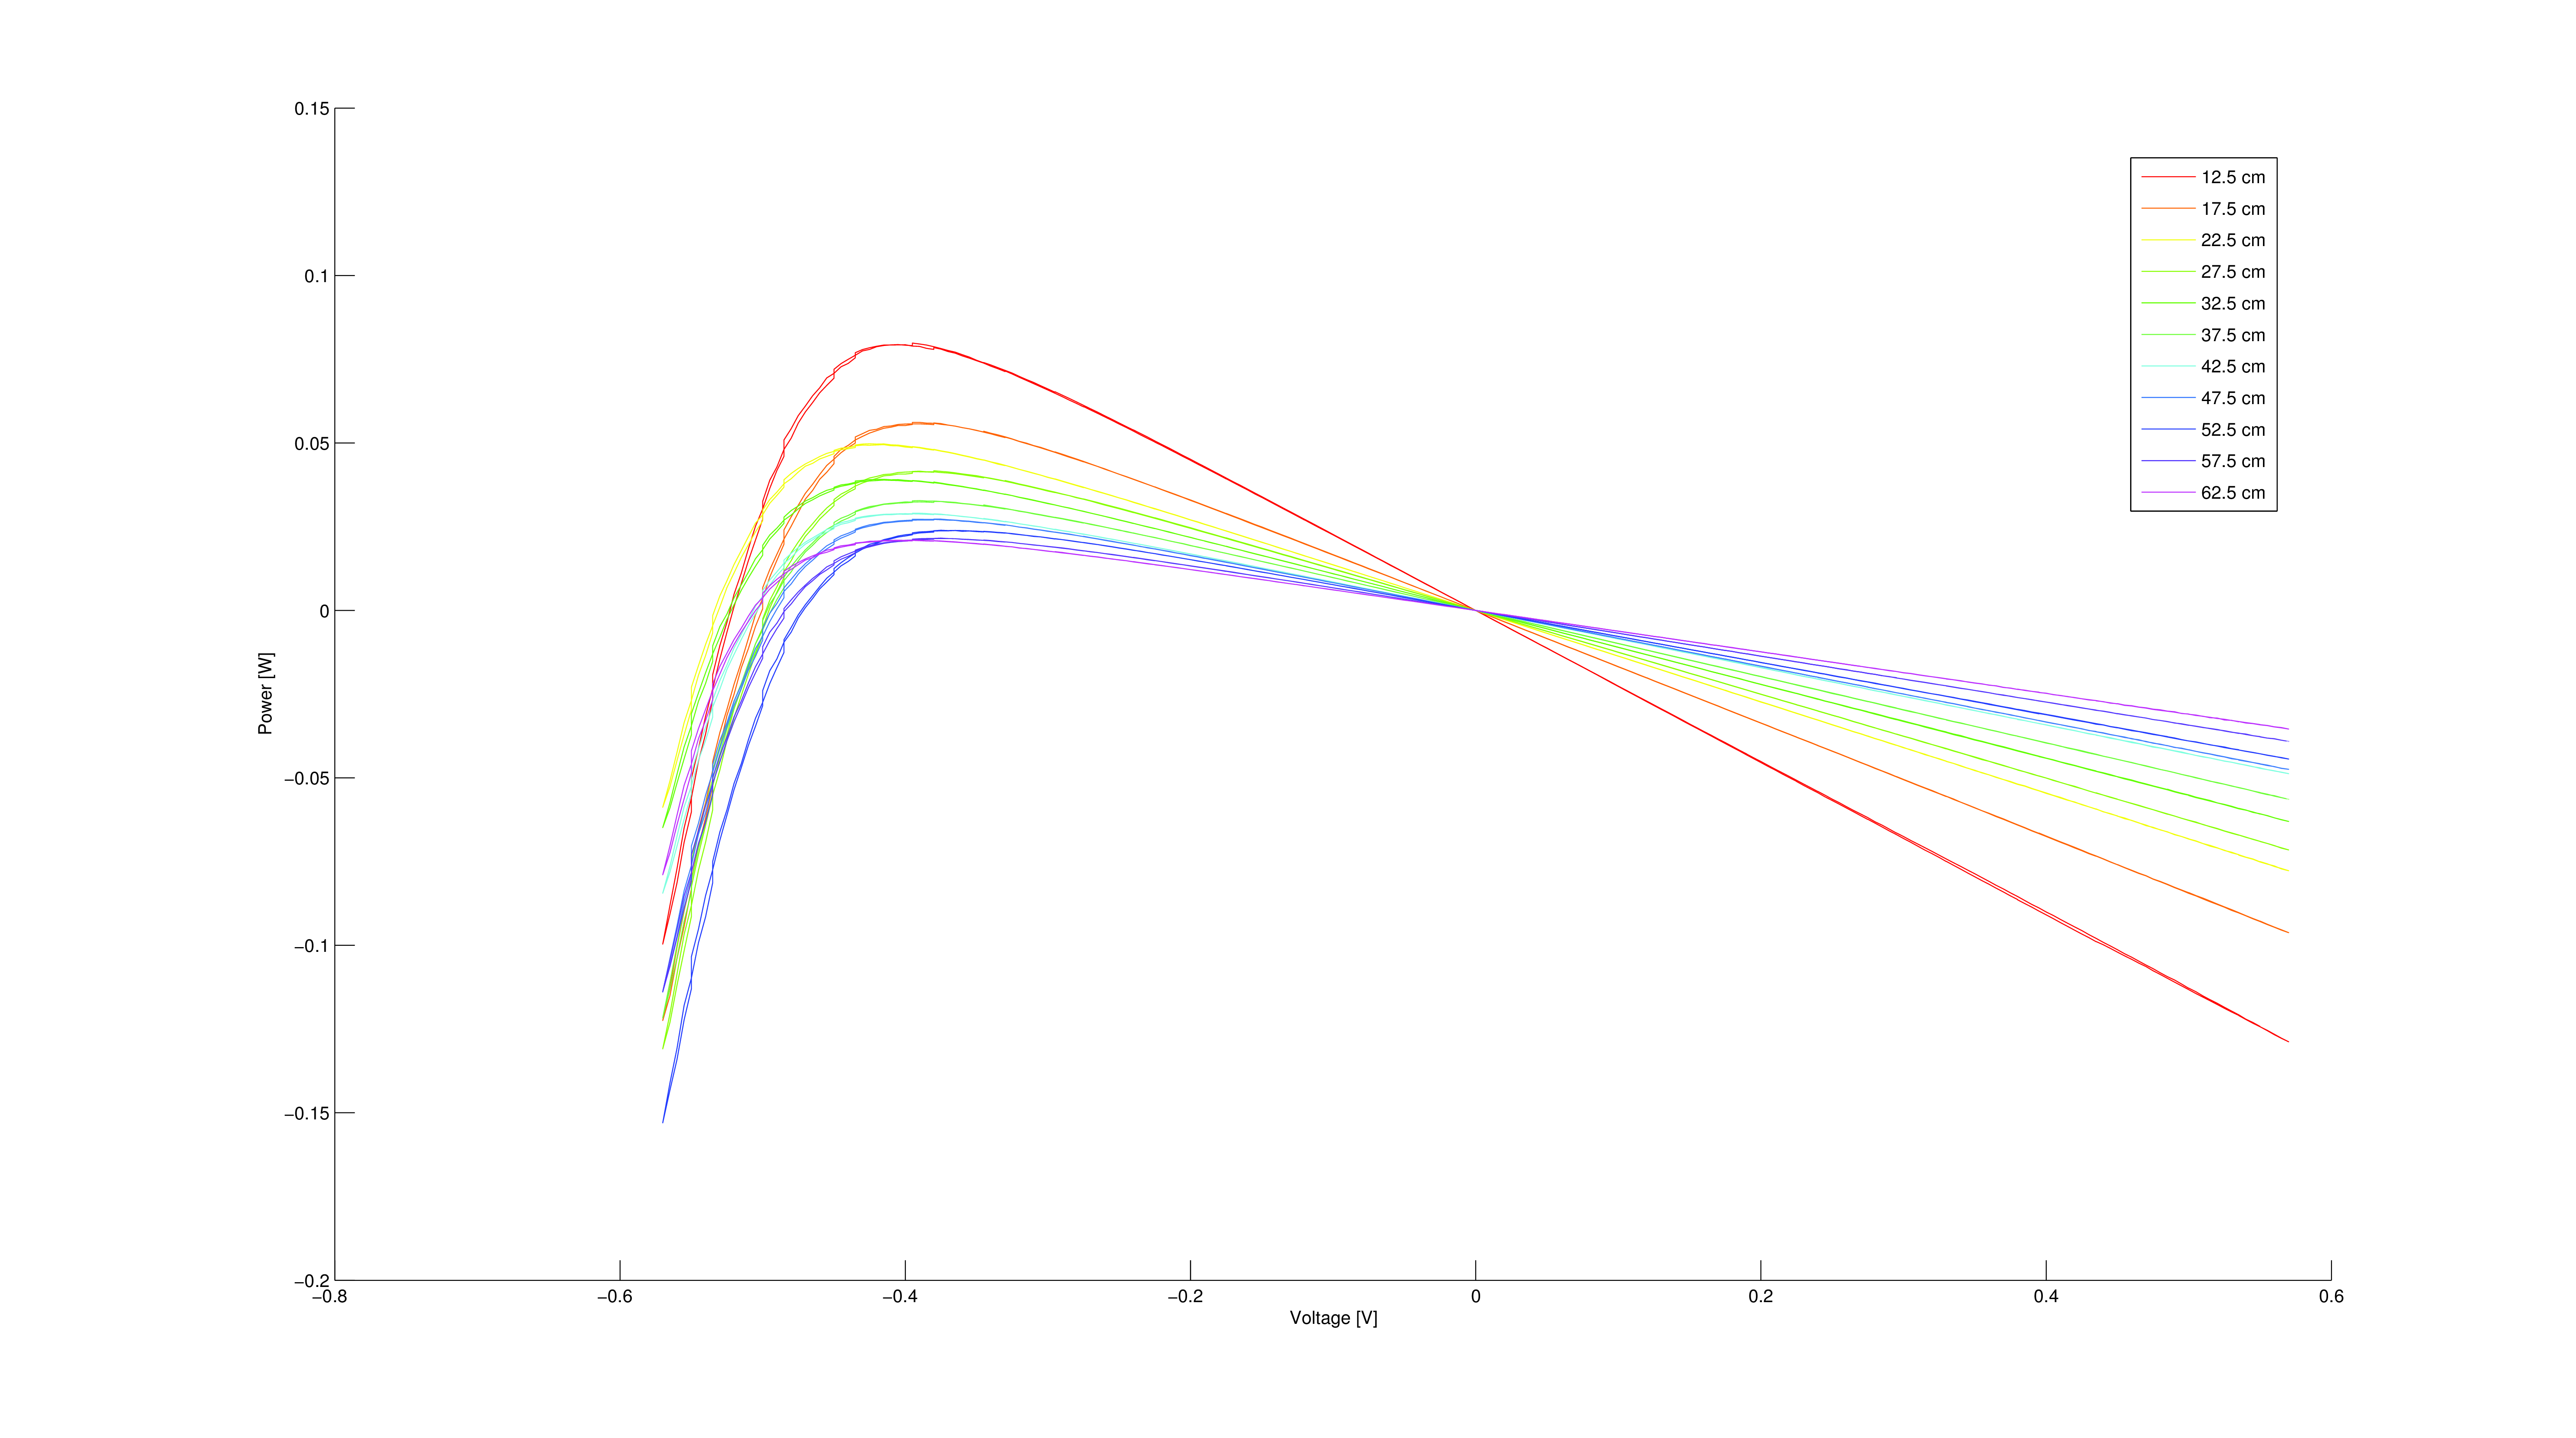
\includegraphics[scale=0.07]{PvsV.png}
  \end{center}
  \caption{Power as function of voltage for different distances from lamp to solar cell.}
  \label{pvsv}
\end{figure}

\begin{figure}[h!]
  \begin{center}
    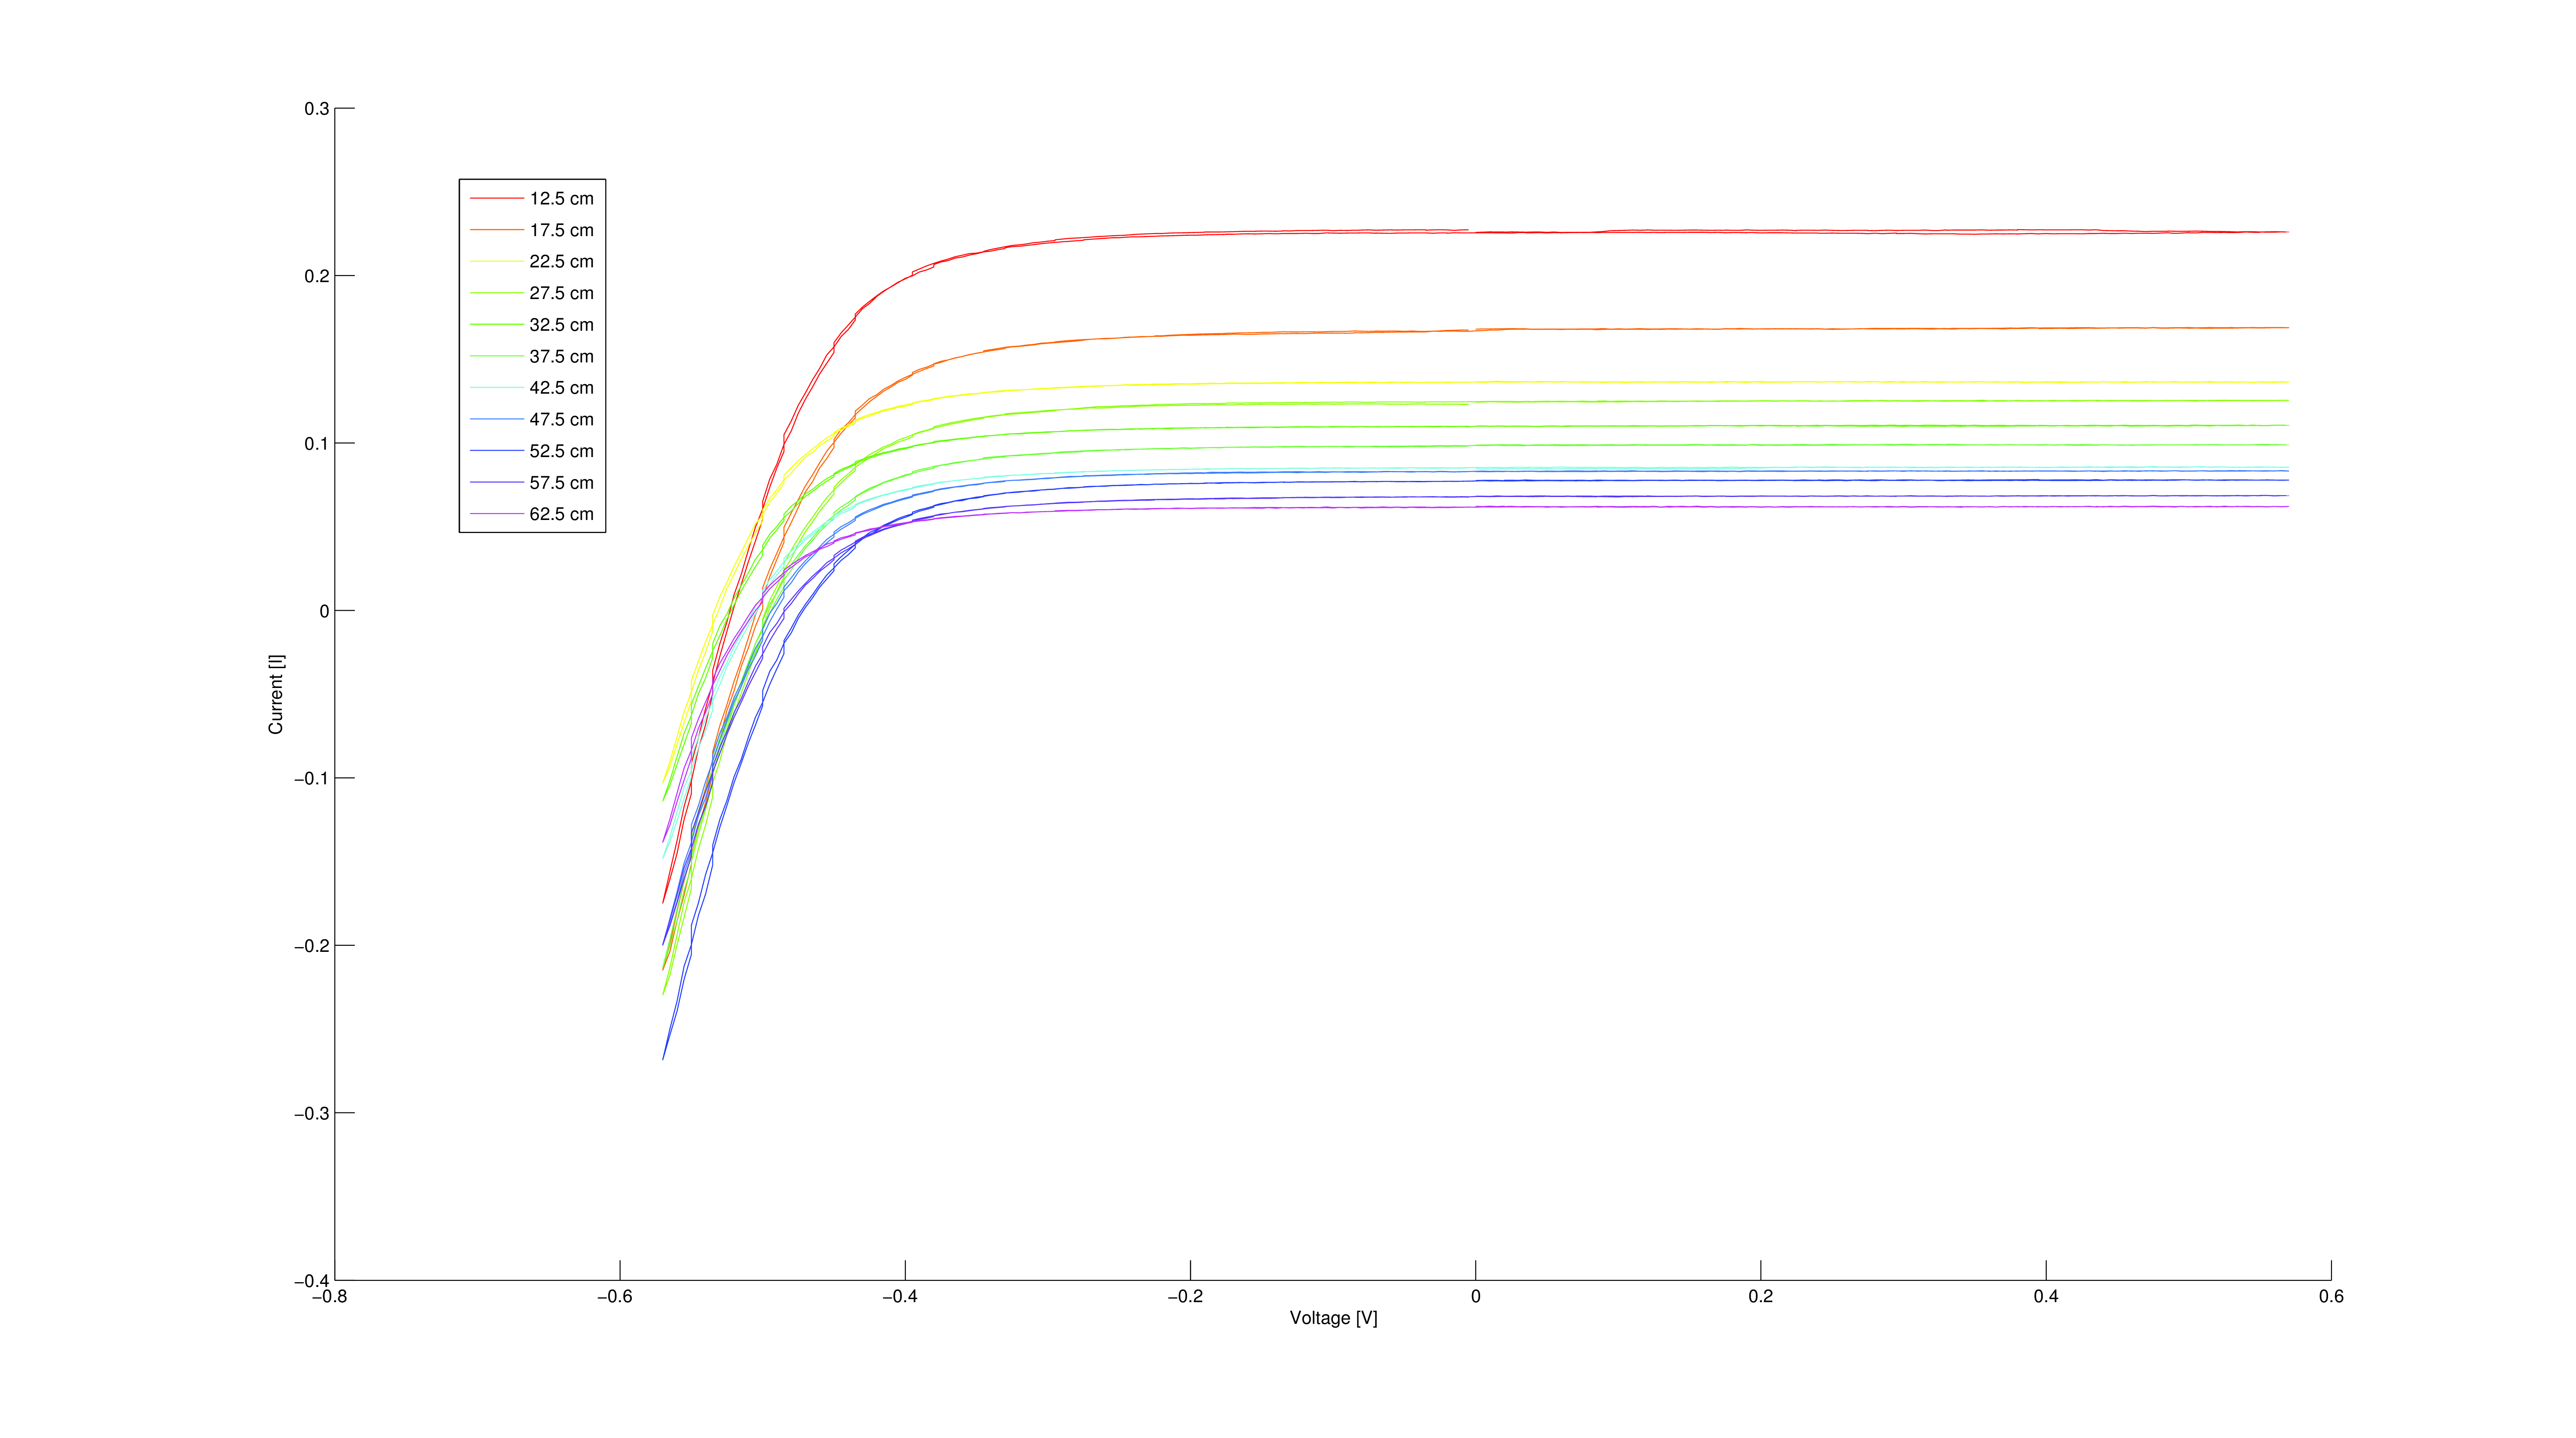
\includegraphics[scale=0.07]{IvsU.png}
  \end{center}
  \caption{Current as function of voltage for different distances from lamp to solar cell.}
  \label{ivsu}
\end{figure}

\begin{figure}[!h]
  \begin{center}
    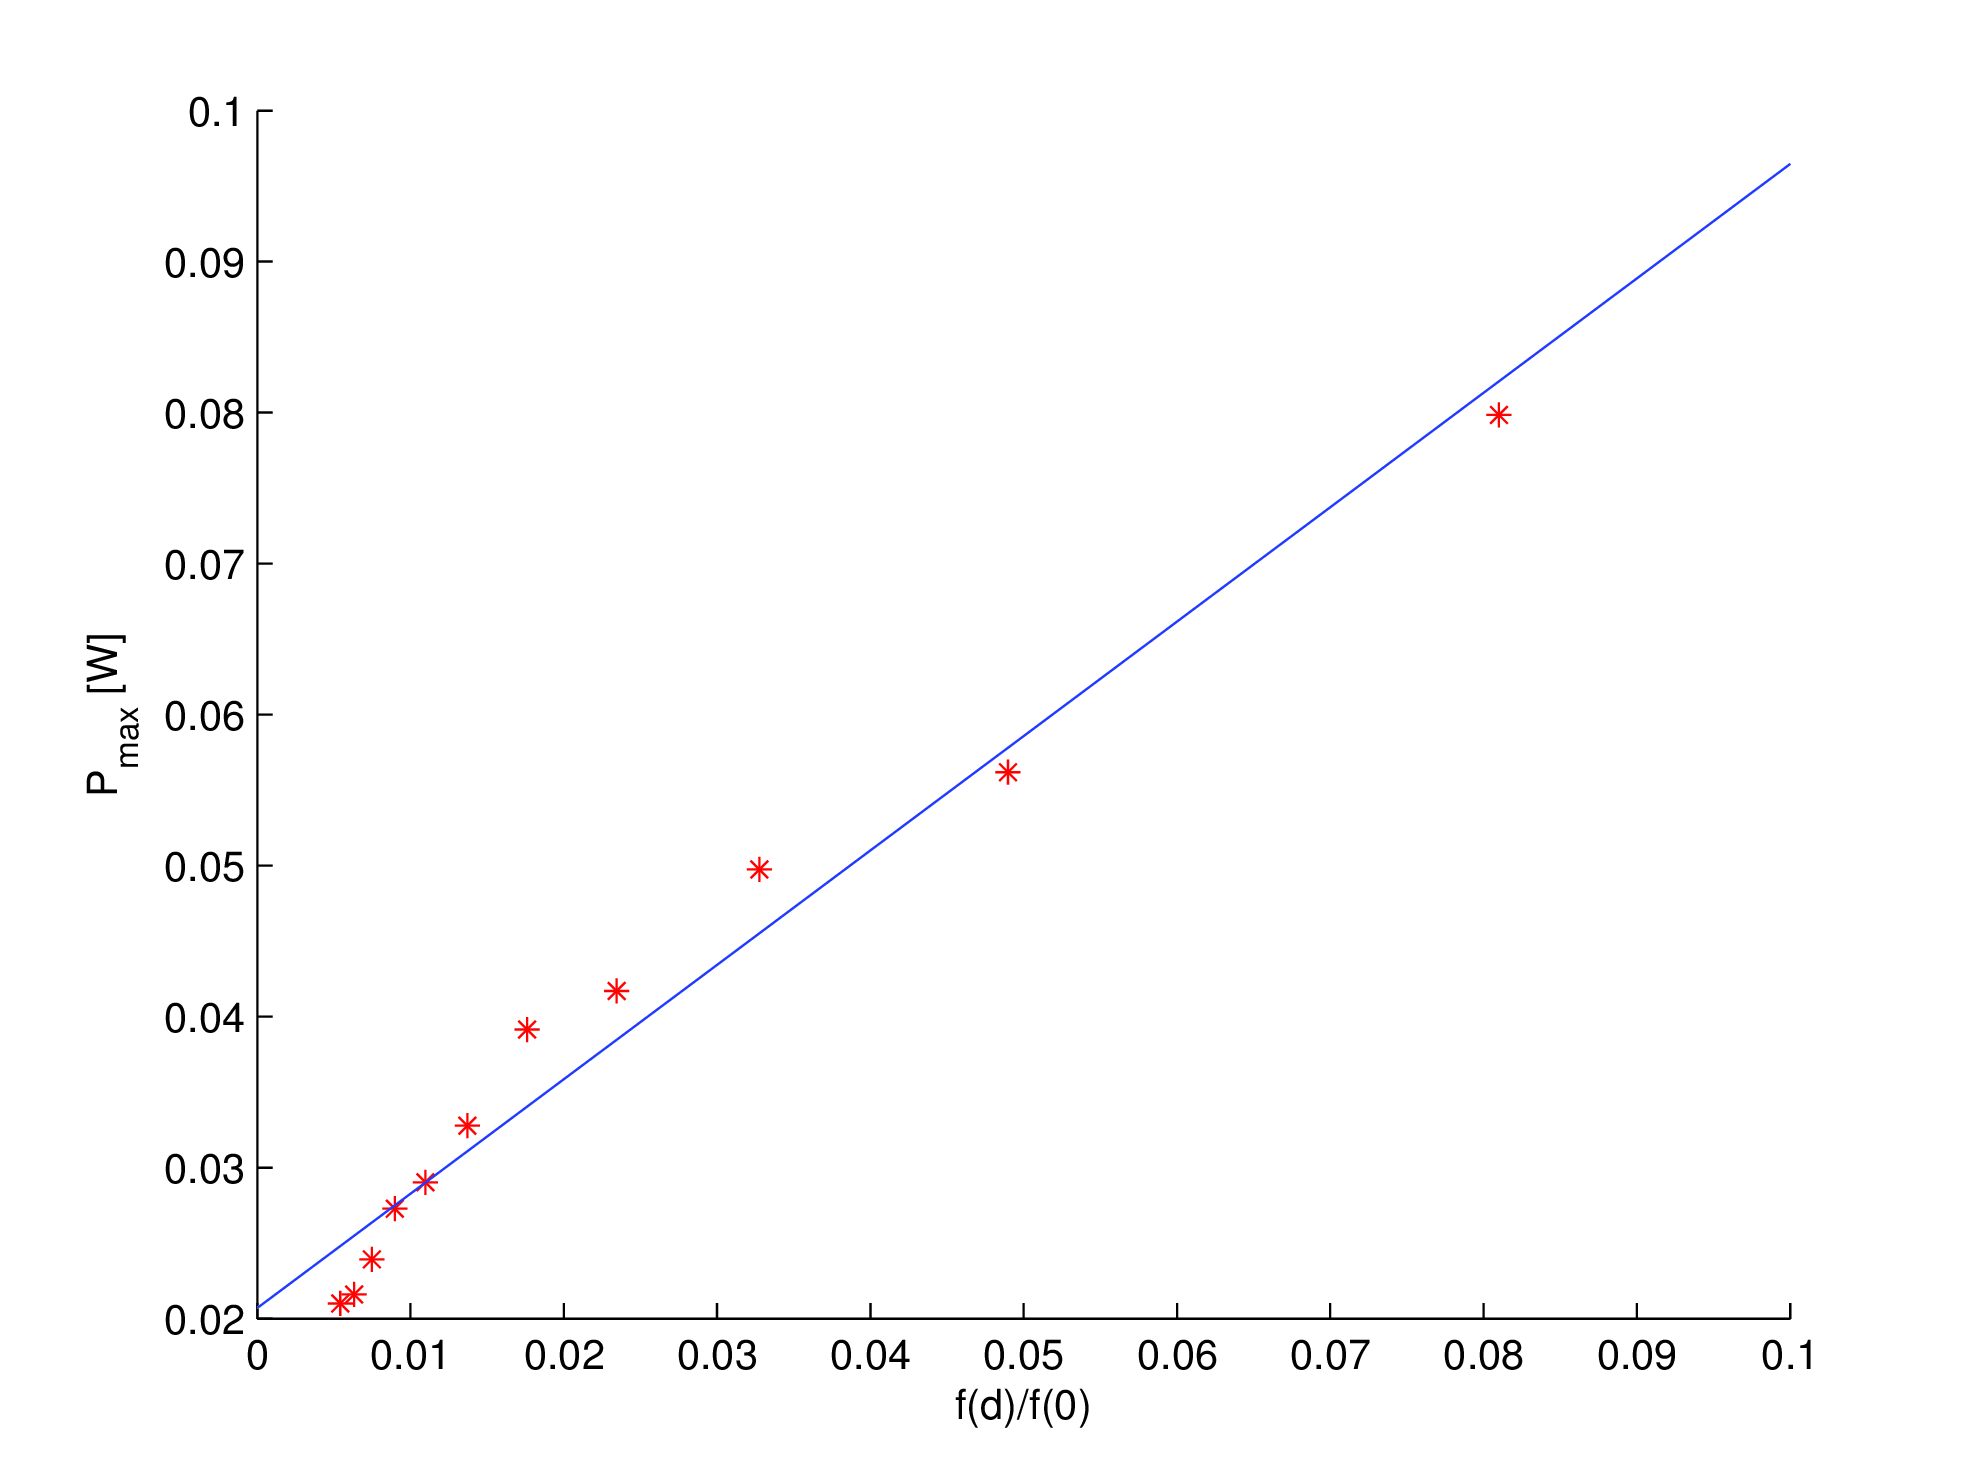
\includegraphics[scale=0.2]{pmaxvsf.png}
  \end{center}
  \caption{Current as function of voltage for different distances from lamp to solar cell.}
  \label{pmaxvsf}
\end{figure}
\vfill
\clearpage

\section{Discussion of the results}

The power delivered to the solar cell should of course satisfy $4\pi R^2\Phi = P$, where $P$ is the effect. (We measured the maximal effect $P_{max}$). Hence, if we fit the curve according to the formula $P_{max}=kf(d)/f(0)$, where $k$ is a proportional constant, $f(d)=\frac{1}{(d+x_0)^2}$ and $d$ the distance from the lamp to the solar cell, we should obtain something that is linear, see figure \ref{pmaxvsf}. We introduced $x_0$ in order to compensate for systematic errors and found that $k=1.76\cdot 10^{-6}$ Wm${}^2$ and $x_0=4.98$ cm, however some differences still remain; some possibly arising from the fact that the lamp is not a perfect sphere. \\

As a way to check the results, consider the following: Approximate the solar cell together with the Power Cassy as a simple circuit, where the solar cell and the Power Cassy has resistance $R_0$ and $R$, respectively. 
By Ohm's law, we know that $U=RI$ and $P=IR^2$. Then, since $U_0=(R+R_0)I$, it follows that $P=RI^2=R\left( \frac{U_0}{R+R_0} \right)^2$.
The voltage at maximum power it therefore given by

\begin{displaymath}
  0=\frac{dP}{dR}=-\frac{U_0^2(R-R_0)}{(R+R_0)^3}\iff R=R_0.
\end{displaymath}

In this case, the voltage is also maximal and given by $U_{max}=R_0I=R_0\frac{U_0}{R_0+R_0}=\frac{U_0}{2}$.
From figure \ref{pvsv}, we see that $U_{max}\approx -0.4$ V and from figure \ref{ivsu}, we see that $U_0\approx -0.5$ V, which does not at all agree with theory. So either the model is too crude or our values are bad.

The most ideal solar cells are of course those whose energy gap coincide with the sun. Now, from \cite{lab_PM}, we know that the maximum efficiency is given by $E_g/(k_BT)\approx 2.3$ and since the temperature of the photosphere is approximately $5800$ K, see \cite{sun}, the best solar cells are those with an energy gap of around $1.15$ eV.
Our solar cell, consisting of Silicone, with an energy gap of around $1.11$ eV at $300$ K is therefore an excellent choice. \\

We considered a $60$ W light bulb with an effective temperature of around $3000$ K. This implies that $E_g/(k_B T)\approx 4.3$, so that \cite{lab_PM} gives us an upper limit on the efficiency to be $25$\%.
Obviously, we do not reach $25$\%, in fact, it ought to be considerably lower. However, to following calculation shows otherwise:
The area of the solar cell was $13.8$ cm${}^2$ and as a rough approximation, assume that the $60$ W light bulb converts all of its energy into radiation. Assume that they are distributed spherically and perfectly aligns with the solar cell. Then, at a distance of $37.5$ cm, $13.8\cdot 60/(4\pi 37.5^2)\approx 0.044$ W will be absorbed by the solar cell.
Thus, by figure \ref{pvsv}, the efficiency is
\begin{displaymath}
  \frac{0.033}{0.044}\approx 0.74,
\end{displaymath}
which is far too high.
The diode equation was used to relate the current $I$ and the voltage $V$ according to

$$I = I_{sat}\left(1-e^{-|q|V/nk_BT}\right) = I_{sat}\left(1-e^{-V/V_0}\right),$$

where we have introduced the variable $V_0 = \frac{nk_BT}{|q|}$. Here $T$ is the surrounding temperature and $n$ the ideality factor. Using non-linear least squares optimization for the observed data from the measurement without illumination, we obtained the best-fit values $I_{sat}=1.78\cdot 10^{-6}$ A and $V_0=0.0498$ V. Figure $\ref{ivsun}$ shows the congruence between theory and experiment. Slight systematic deviation can be seen for positive voltage due to small currents in the backward bias. \\

We found the ideality factor to be $n = \frac{|q|V_0}{k_BT} = 1.93$, which can be compared to $1$, the value of an ideal diode. The occurrence of recombination of electrons and holes could account for some discrepancy. Furthermore, due to the presence of ambient light, a current could be measured even at zero bias. \\

We also note that our methodology was not free of errors. We approximated the distribution of the light from the lamp as spherical, while in reality a lampshade focused the light into a cone.

\section{Conclusions}
The effectiveness of a solar cell consisting of Silicon has been measured, however, the results does not seem to agree with known theory except for agreement with the diode equation and the fact that the obtained power decreased with increasing distance.

\begin{thebibliography}{9}
\bibitem{kittel} C. Kittel, \emph{Introduction to Solid State Physics}, 8th Edition, Hoboken, NJ: John Wiley \& Sons, 2005, pp. 190.
\bibitem{lab_PM} R. Fors, \emph{Photovoltaic effect: Diode IV-characteristic}, KTH Condensed Matter Physics, 2005.
\bibitem{sun} Wikipedia: Sun. Available at \url{http://en.wikipedia.org/wiki/Sun}.
\end{thebibliography}

\end{document}
